\section{Experimental Setups}
\label{sec:experimental-setups}

\begin{figure*}[t]
\centering
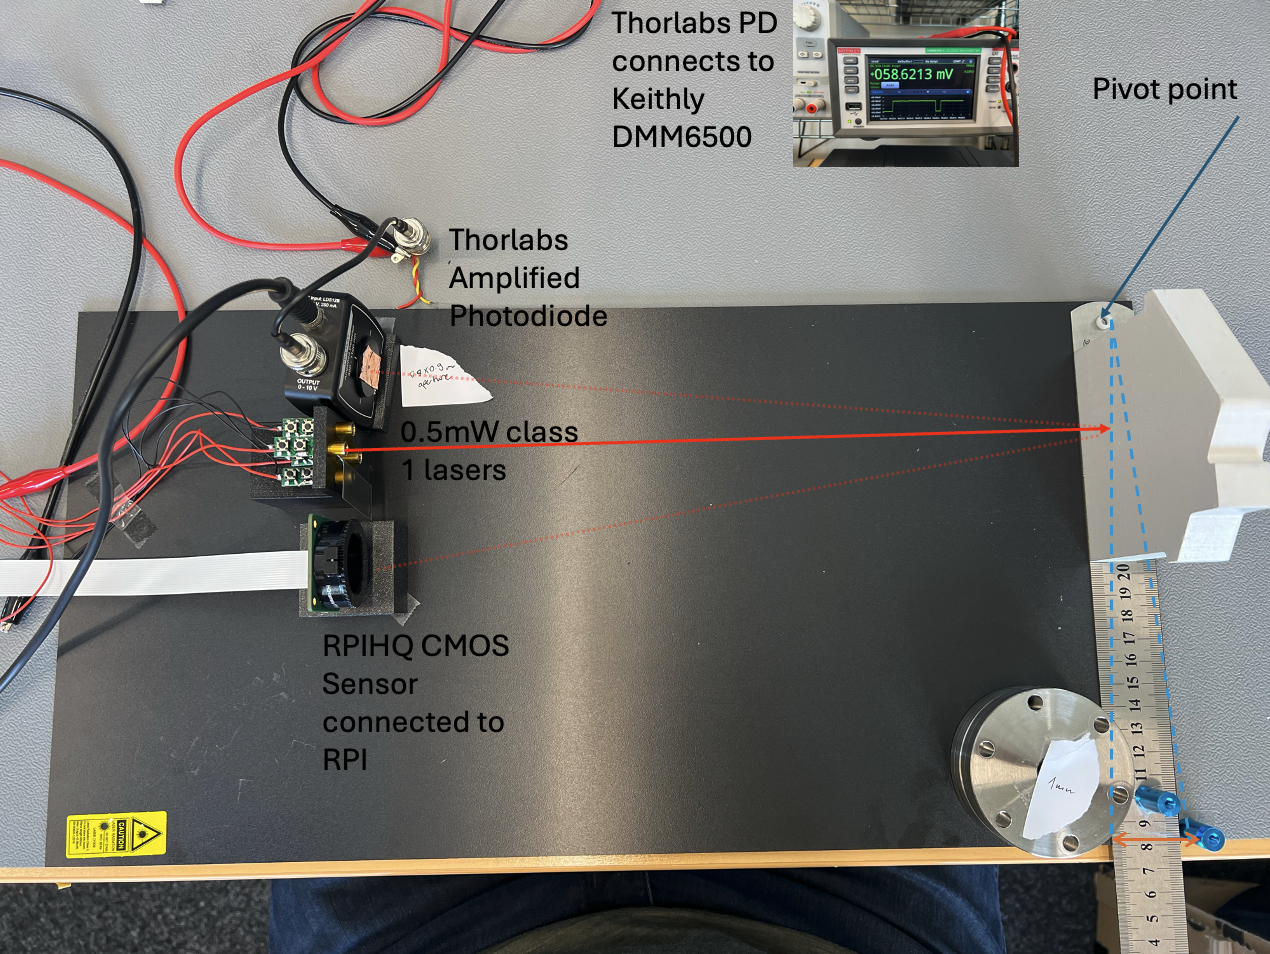
\includegraphics[width=\textwidth]{figures/impl/camera_setup.png}
\caption{A laser is pointed at a painted wooden surface. A multimeter measured the current from a masked photodiode. A RPI HQ camera is used as a reference to visualise the speckle pattern.}
\label{fig:cam1}
\end{figure*}


\begin{figure*}[t]
\centering
\includegraphics[width=\textwidth]{figures/eval/typical_setup.png}
\caption{Photo of the experimental configuration with the piezo disc.}
\label{fig:setup}
\end{figure*}


\begin{figure*}[t]
\centering
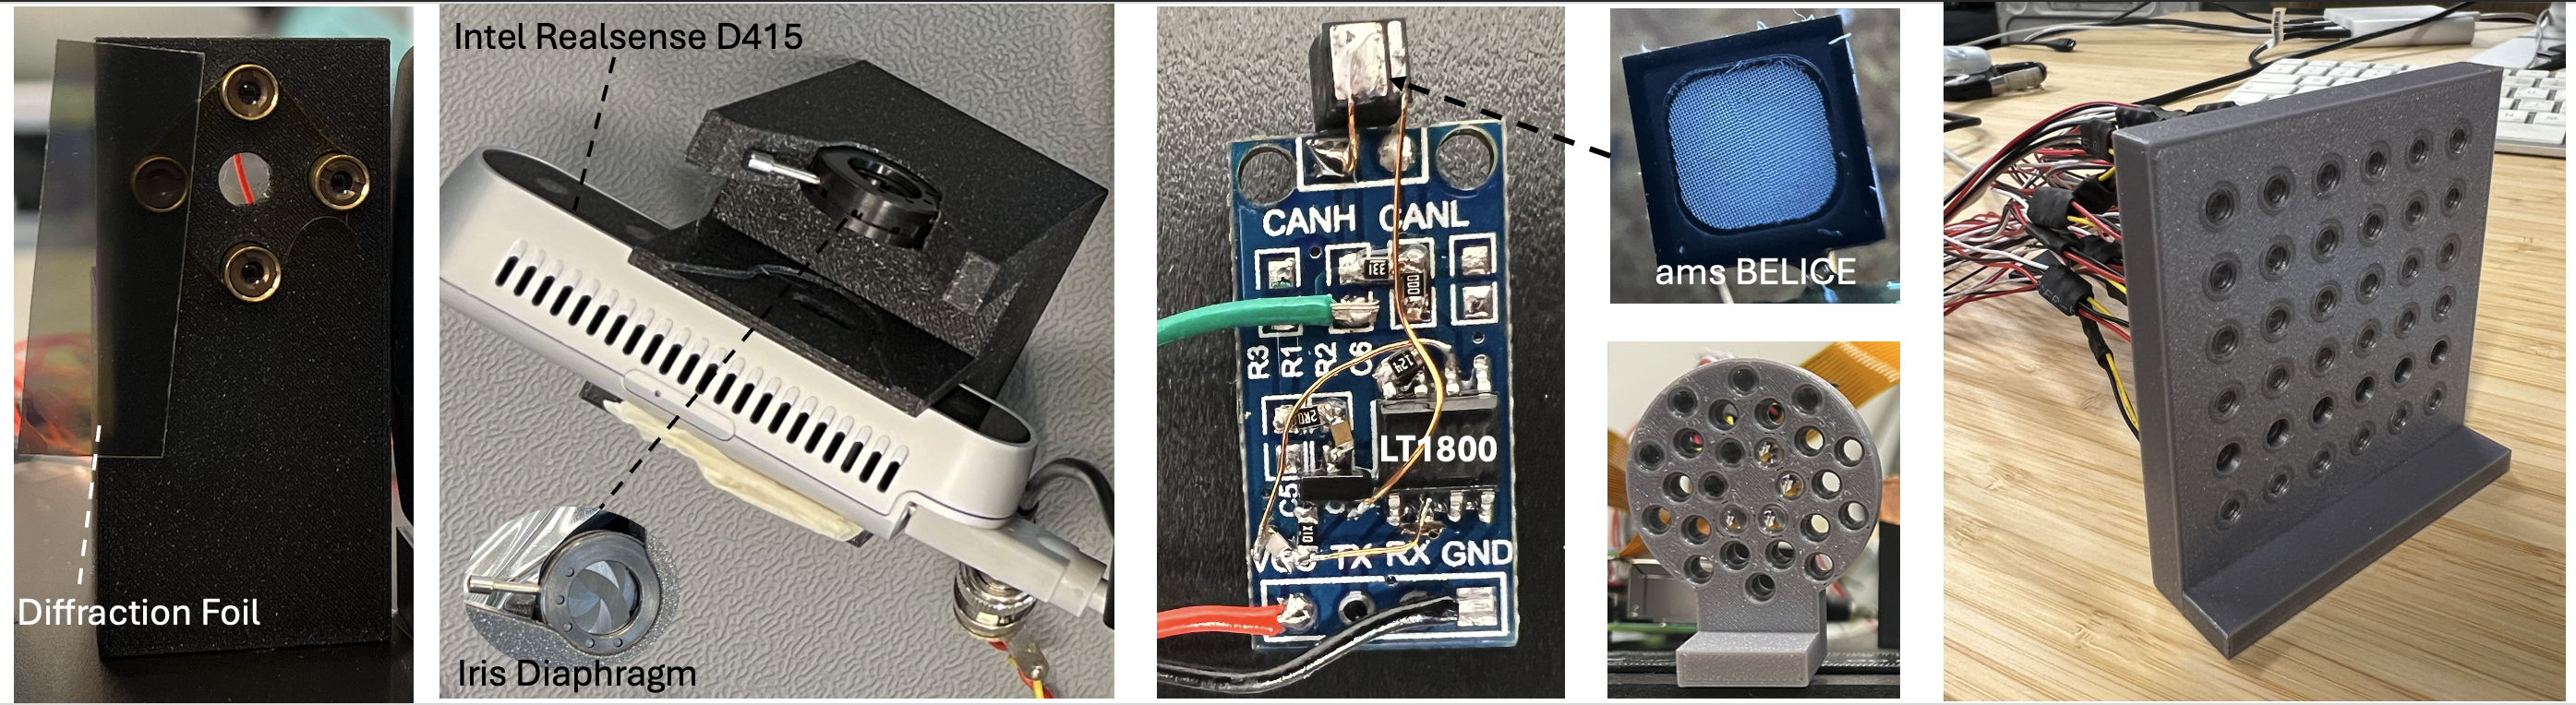
\includegraphics[width=\textwidth]{figures/eval/lasers}
\caption{The different laser setups used from left to right: Red laser for initial emulation experiments, Realsense 415 dot projector with iris, reverse engineered Realsense dot projector and driver circuit, discrete circular and square IR laser arrays.}
\label{fig:lasers}
\end{figure*}
